\documentclass[english]{article}
\usepackage{babel}
\usepackage{blindtext}
\usepackage{microtype}
\usepackage{color}
\usepackage{amsmath}
\usepackage{graphicx}
\usepackage{ragged2e}

\begin{document}

\title{\Large{\textbf{Air Cargo Optimization}}}
\author{DDS - RWTH Business School}
\date{April 30th, 2018}

\maketitle

\begin{flushleft}
\textbf{\underline{\large{Introduction}}}:
$\newline$

An Airport needs to plan the cargo movement so that all shipments catch their connecting flights (or road connection). Air cargo shipments are transported in so-called unit load devices (ULDs). A ULD contains many shipments which need to go to different destinations and hence the incoming ULDs are broken down and re-built according to the flights the shipments have to catch. The goal of the optimization proccess is buildup all ULDs as soon as possible to make the connections

$\newline$
\textbf{\underline{\large{Process description}}}:
$\newline$

ULDs are unloaded from an aircraft by the ground handling agent and placed in their respective drop zones. Each ULD has an arrival time. From the drop zone the ULDs need to be transported to a breakdown zone (BD zone), which are located at different places of the airport, have different capacity and handling times within the zone.


\noindent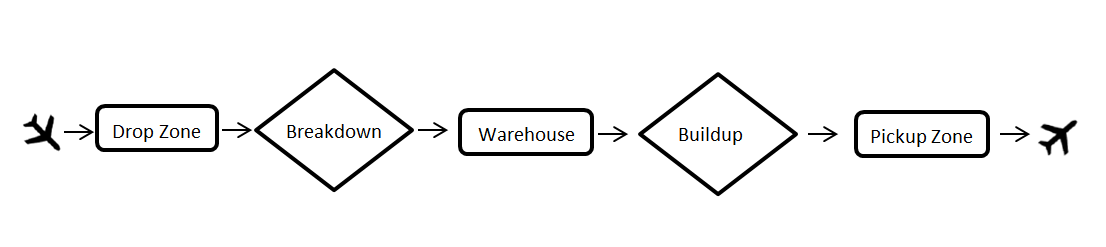
\includegraphics[width=13cm]{1_process.png}\qquad

$\newline$
Within the BD zone the decision needs to be taken in which order the ULDs should be unpacked.  ULDs need to be broken down early enough, so all shipments can make their connections or promised pick-up time. When the shipments are unpacked, they are sent to the storage warehouse (WH) which is fully automated and with the assumption, that there are never capacity issues in the storage WH.
$\newline$


In the next step the shipments are built up again to ULDs depending on their connecting flight. This is done within a buildup zone (BU zone). A departing aircraft type has a link to a specific BU zone. As soon as enough stock is available in the storage WH to build up one ULD for a specific aircraft, these can be requested to be provided to the BU zone.
$\newline$

Each BU zone consists of multiple work stations. At each work station one ULD can be built up at the same time. The shipments are provided from the storage WH to the chosen workstation. If the building up of two ULDs for the same aircraft are planned at one work station, it is not allowed to build up a ULD for a different aircraft in between, even if there is some idle time.
$\newline$

\noindent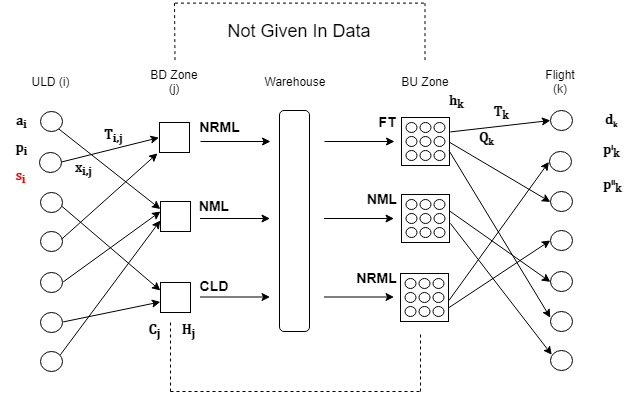
\includegraphics[width=13cm]{Aircargo_overall.png}\qquad

\pagebreak

\begin{table}[h!]
  \begin{center}
    \caption{Drop Zone}
    \label{tab:table1}
    \begin{tabular}{l|c|c} % <-- Alignments: 1st column left, 2nd middle and 3rd right, with vertical lines in between
      \textbf{Name} & \textbf{Workstations} & \textbf{Sequence}\\
      \hline
       & & \\
      DZ NRML-1 & 6 & 1\\
      DZ NRML-2 & 4 & 2\\
      DZ NML-1 & 3 & 3\\
      DZ CLD-1 & 5 & 4\\
    \end{tabular}
  \end{center}
\end{table}

\begin{table}[h!]
  \begin{center}
    \caption{Break Down Zone}
    \label{tab:table1}
    \begin{tabular}{l|c|c|c|c} % <-- Alignments: 1st column left, 2nd middle and 3rd right, with vertical lines in between
      \textbf{Name} & \textbf{Workstations} & \textbf{Sequence} & \textbf{ToWH} & \textbf{HandTimePerULD}\\
      \hline
       & & & & \\
      B BD NRML-1 & 33 & 1 & 0:30 & 0:24\\
      B BD NRML-2 & 10 & 2 &  0:25 & 0:24\\
      BD NML-1 & 4 & 3 &  0:40 & 0:13\\
      BD CLD-1 & 8 & 4  &  0:30 & 0:17\\
      BD NRML-1 & 5 & 5  &  0:30 & 0:20\\
      BD NML-2 & 3 & 6  & 0:25 & 0:13\\
      BD NRML-2 & 6 & 7  & 0:40 & 0:20\\
      BD NRML-3 & 3 & 8  & 0:40 & 0:20\\
      BD CLD-2 & 5 & 9  & 0:30 & 0:17\\
      BD NML-3 & 5 & 10  & 0:25 & 0:20\\
      BD NRML-4 & 3 & 11  & 0:30 & 0:13\\
      BD CLD-4 & 1 & 12  & 0:40 & 0:15\\
    \end{tabular}
  \end{center}
\end{table}

\pagebreak

\textbf{\underline{\large{Arrival}}}:

Let each ULD ${\color{black}i\in{\color{black}I = \{1,2,3,\dots,n\}}}$

${\color{black}a_{i}}$ - Arrival time of each ULD ${\color{black}i}$

$\textcolor{black}{s_{i}}$ - Idle time spent by ULD i at drop zone

$\textcolor{black}{p_{i}}$ - Priority of ULD i

$\newline$

\textbf{\underline{\large{Break Down (BD) Zones}}}: $\textcolor{black}{j\in J = \{1,2,3,\dots,m\}}$

$\newline$

\textbf {From the drop zone the ULDs need to be transported to a breakdown zone (BD zone), which are located at different places of the airport, have different capacity and handling times within the zone.}

\noindent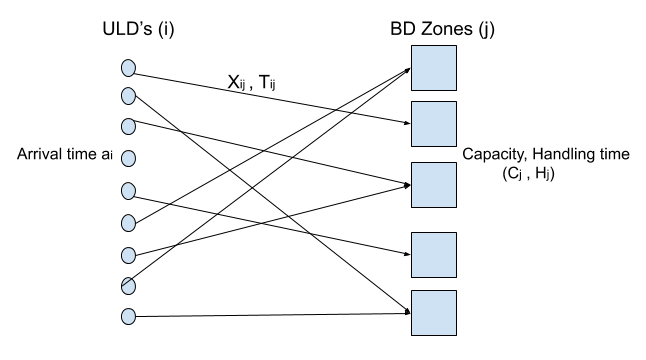
\includegraphics[width=12cm]{BDzone.png}\qquad

$\textcolor{black}{x_{ij}\in\{0,1\},\forall {i \in I, j \in J}}$ - denotes if ULD $i$ is
assigned to BD zone $j$ or not.


$\textcolor{black}{t_{j}}$ - Time taken to transport an ULD to BD
zone \textcolor{black}{$j$}

$\textcolor{black}{C_{j}}$ - Capacity of each BD Zone \textcolor{black}{$j$}

$\textcolor{black}{H_{j}}$ - Handling time of a ULD from in BD zone \textcolor{black}{$j$}

$\textcolor{black}{a_{i}+s_{i}+{\displaystyle \sum_{i,j\in E}x_{i,j}T_{j}}}$ - gives the
Arrival time of ULD \textcolor{black}{$i$} to its BD zone \textcolor{black}{$j$}

$\textcolor{black}{\displaystyle \sum_{i,j\in E}x_{i,j}}$ $\leq{C_{j}}$ , $\forall{j \in J}$ - Capacity constraint needs to be checked from time to time

\pagebreak

\textbf{\underline{\large{Warehouse}}}:

\textbf {When the shipments are unpacked, they are sent to the storage warehouse (WH) which is fully automated and with the assumption, that there are never capacity issues in the storage WH. In a next step the shipments are built up again to ULDs depending on their connecting flight. A departing aircraft type has a link to a specific BU zone, so with the provided information which aircraft the shipment should go on, the BU zone is known.
}

$\newline$

$\textcolor{black}{T_{j}^{\prime}}$ - Time taken to transport shipment from BD zone \textcolor{black}{$j$} to Warehouse

$\textcolor{black}{W_{k}}$ - Time at which, all shipments for a new Flight k are requested

$\textcolor{black}{T_{k}^{\prime}}$ - Transport time from Warehouse to BU Zone for all shipments of Flight \textcolor{black}{$k$}

$\newline$

\textbf{\underline{\large{Build Up (BU) Zone}}}:

$\newline$

$\textcolor{black}{B_{k}}$ - Time taken to Build up ALL new ULDs for flight \textcolor{black}{$k$}

$\textcolor{black}{d_{k}}$ - Departure time of a flight \textcolor{black}{$k$} must be ready (given)

$\textcolor{black}{T_{k}}$ -Transport time from BU to Flight \textcolor{black}{$k$} (given)

$\textcolor{black}{p_{k}^{\prime}}$ - Default processing time of flight \textcolor{black}{$k$} (given)

$\textcolor{black}{p_{k}^{\prime\prime}}$ - Pre processing time of flight \textcolor{black}{$k$} (given)

$\textcolor{black}{W_{k}}$ + $\textcolor{black}{T_{k}}$ +${T_{k}^{\prime}}$+ $\textcolor{black}{B_{k}}$ + $\textcolor{black}{p_{k}^{\prime}}$ + $\textcolor{black}{p_{k}^{\prime\prime}}$ $\leq$ $\textcolor{black}{d_{k}}$ //Constraint respecting Flight time

$\newline$

\noindent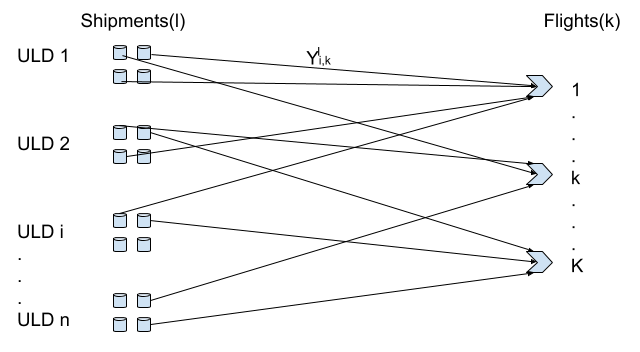
\includegraphics[width=12cm]{BUzone.png}\qquad

\pagebreak

Let $\textcolor{black}{Y_{i,k}^{l}}$ $\in\{0,1\}$ - depending on whether shipment l going to flight k is in ULD i or not.

$\textcolor{black}{w_{l}}$ - Weight of each shipment \textcolor{black}{$l$} (given)

$\textcolor{black}{Q_{k}}$ - Total weight of shipments going via flight \textcolor{black}{$k$} (summation of $\textcolor{black}{w_{l}}$)(given)

$\textcolor{black}{\displaystyle \sum_{i\in I} \sum_{l\in L}Y_{i,k}^{l}}$$\textcolor{black}{w_{l}}$ = $\textcolor{black}{Q_{k}}$ , $\forall{k}$ - Respecting assigned shipment weight to Flights \textcolor{black}{$k$}

$\textcolor{black}{\displaystyle \sum_{i\in I} \sum_{l\in L} \sum_{k\in K}Y_{i,k}^{l}}$ - N // Total no of shipments

All shipments of flight k, should reach be available before time $\textcolor{black}{W_{k}}$:

$\textcolor{black}{a_{i}+s_{i}+{\displaystyle \sum_{i,j\in E}x_{i,j}T_{j}}}+{T_{j}^{\prime}}+{H_{j}}$ $\leq$ ${W_{k}}$ + (1-${Y_{i,k}^{l}}$)M, $\forall{i,k,l}$ // Time constraint for every shipment.

$\newline$

\textbf{\large{Objective Function}}: Minimizing the maximum slack
$\newline$

$\textcolor{black}{Min(Max(  s_{i}}+{W_{k}}$))

\end{flushleft}

\end{document}
